\section{Third Member}
This is the section dedicated to one of the team members, and it should be written individually . It can include a range of things; first subsection is a space for you to point out the strengths and weaknesses of the module, including complaints about the module coordinator Max Wilson. The second section should have a selfie image with Max! The last part of it is the most important one. You will need to write a paragraph about what you have learned in this module. You can write it in \textbf{Bold} if you want or you can use other fonts. 

Please do not forget:
\begin{itemize}
	\item First paragraph should have your comments about the module
	\item Second one, a selfie img with Max
	\item Last one, what you learned in this module.
\end{itemize}

\subsection{Comments about the module}
\textbf{This module has been quite enjoyable with the practical aspects of it. It is also helpful that practise exam questions have been given. The module is however very fast paced with a lot of content to go through each lecture.}  

\subsection{Selfie with Max}

\begin{figure}[h]
\caption{Selfie with Max}
\centering
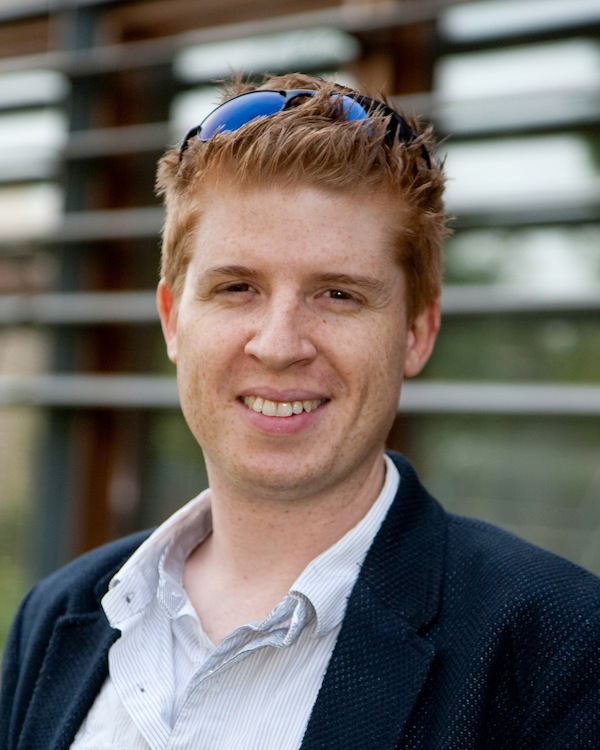
\includegraphics[width=0.5\textwidth]{max.jpg}
\label{fig:selfie}
\end{figure}

 My selfie with Max is in  Figure~\ref{fig:selfie}.

\subsection{What I have learned in this module}
Interesting to learn about the different types of UML and how they are used. Learnt about the different stages of the software engineering process. I've understood the difference between requirements and specifications and how to use UML to differentiate between the two. Also learnt about LaTeX and how to create stylish documents!

